\chapter{\mbox{Thực nghiệm và đánh giá kết quả}} \label{chapter04}


\section{Môi trường thực nghiệm}
Để đánh giá hiệu quả của mô hình phân loại được đề xuất, chúng tôi cài đặt chương trình nhận dạng và phân loại ảnh bệnh trên lá cam bằng ngôn ngữ lập trình Python [Rossum, 1991], rút trích các đặc trưng SIFT, Color bằng thư viện OpenCV [Bradski \& Kaehler, 2012], HOG bằng thư viện scikit-image \cite{scikit-image}, GIST bằng thư viện Pyleargist [Grisel, 2009] và đặc trưng ResNet bằng thư viện Keras [Chollet, 2015]. Thư viện scikit-learn [Cournapeau, 2007] được sử dụng để huấn luyện mô hình phân loại bệnh. Trong phần \ref{sec:thuc-nghiem-phan-loai} thực nghiệm phân loại, chúng tôi cũng muốn so sánh mô hình đề xuất SVM với mô hình KNN để kiểm chứng như trong bài nghiên cứu \cite{kim12012comparing} là đúng sự thật.\par
Thực nghiệm được thực hiện trên máy tính cá nhân, cài đặt hệ điều hành Linux Ubuntu 18.04 LTS, bộ vi xử lý Intel\textsuperscript{\textregistered} Core i5-3337U, 1.8GHz, 4 nhân và bộ nhớ RAM 8 GB.

\section{Thực nghiệm phân loại} \label{sec:thuc-nghiem-phan-loai}
\subsection{Chuẩn bị tập dữ liệu kiểm thử}
Mô hình sau khi được huấn luyện ở phần \ref{sec:training-model} được sử dụng để phân loại trên tập dữ liệu kiểm thử, bước rút trích các đặc trưng tạo ra tập dữ liệu dạng bảng, có 142 dòng, mỗi dòng tương là ảnh lá bệnh có 103124 chiều, đã được xáo trộn trước khi đưa vào mô hình phân loại. Bảng \ref{tab:statistics-label-test-dataset} thống kê số lượng mẫu của tường lớp trong tập dữ liệu kiểm thử.

\begin{table}[h]
\caption{Thống kê số lượng mẫu trong tập dữ liệu thử}
\centering
\begin{tabular}{|c|l|c|c|}
\hline 
\textbf{STT} & \textbf{Tên loại bệnh} & \textbf{Nhãn trong hệ thống} & \textbf{Số lượng nhãn/lớp}\\ [0.5ex] \hline \hline
1 & Ghẻ nhám & 0 & 30 \\
2 & Lá khỏe & 1 & 28 \\ 
3 & Rầy phấn trắng & 2 & 30 \\
4 & Vàng lá gân xanh & 3 & 27 \\
5 & Vàng lá thối rễ & 4 & 27 \\ \hline
\multicolumn{2}{|c|}{\textbf{Tổng cộng:}} & 5 & 142 \\ \hline
\end{tabular}
\label{tab:statistics-label-test-dataset}
\end{table}
 
\subsection{Kết quả thực nghiệm}
Chúng tôi sử dụng tập dữ liệu kiểm 142 dòng để tiến hành kiểm thử dựa trong mô hình đã được huấn luyện trước đó. Bảng \ref{tab:test-dataset} thống kê số nhãn trong mỗi lớp, kết quả phân loại đúng và sai của mô hình. Kết quả cho thấy bệnh vàng lá thối rễ cho kết quả phân loại chính xác tuyệt đối do bệnh có thể dễ dạng nhận dạng bằng màu vàng nỗi bậc trên toàn bộ phiến lá, khác với bệnh rầy phấn trắng, bệnh khó nhận biết với đóm nhỏ màu nâu ở phần mặt trên của lá với bệnh ghẻ nhám hoặc lá khỏe, để nhận biết chính xác thì cần phải chụp ở phần dưới của mặt lá vì có nhiều lông sáp hình dạng tròn.\par

\begin{table}[h]
\caption{Thống kê mẫu phân loại đúng và sai trên tập dữ liệu kiểm thử của mô hình SVM}
\centering
\begin{tabular}{|c|l|c|l|l|}
\hline
\textbf{STT} & \textbf{Tên loại bệnh} & \textbf{Mẫu kiểm thử} & \textbf{Phân loại đúng} & \textbf{Phân loại sai}\\ [0.5ex] \hline \hline
1 & Ghẻ nhám & 30 & 26 \emph{(86.66\%)} & 4 \emph{(13.33\%)} \\
2 & Lá khỏe & 28 & 27 \emph{(96.42\%)} & 1 \emph{(3.57\%)}\\
3 & Rầy phấn trắng & 30 & 25 \emph{(83.33\%)} & 5 \emph{(16.66\%)}\\
4 & Vàng lá gân xanh & 27 & 24 \emph{(88.88\%)} & 3 \emph{(11.11\%)}\\
5 & Vàng lá thối rễ & 27 & 27 \emph{(100\%)} & 0 \emph{(0\%)}\\ \hline
\multicolumn{2}{|c|}{\textbf{Tổng cộng:}} & 142 & 129 \emph{(90.84\%)} & 13 \emph{(9.15\%)} \\ \hline
\end{tabular}
\label{tab:test-dataset}
\end{table}

Hình \ref{fig:predict-result} là kết quả phân loại với 3 ảnh là các loại bệnh khác nhau, được phân loại chính xác với tổng thời gian phân loại là 1.6 phút, tương ứng mỗi hình cho thời gian phân loại là 32 giây, đạt mục tiêu đề ra của đề tài là phân loại bệnh trên lá cam.

\begin{figure}[!htp]
	\centering
	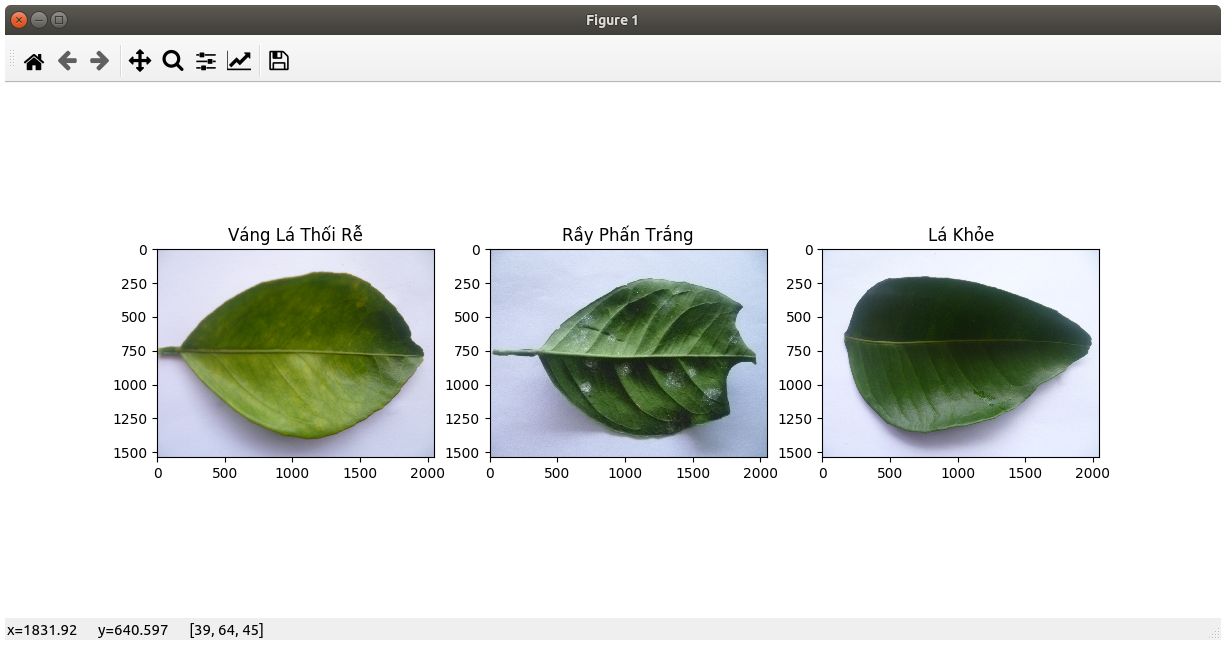
\includegraphics[width=0.9\textwidth]{predict-result}
	\caption{Kết quả phân loại của mô hình SVM}
	\label{fig:predict-result}
\end{figure}

Chúng tôi cũng tiến hành huấn luyện mô hình máy học KNN để so sánh với mô hình máy học SVM do chúng tôi đề xuất, bộ tham số của hai mô hình cũng được tìm dựa trên nghi thức kiểm tra chéo từ tập dữ liệu huấn luyện. Mô hình máy học KNN phân lớp dữ liệu dựa trên khoảng cách Euclidean, tức là một điểm dữ liệu mới sẽ được gán nhãn dựa trên K láng giềng gần nó nhất. Bảng \ref{tab:so-sanh-knn-svm} cho thấy trong trường hợp này mô hình máy học SVM cho kết quả tốt hơn mô hình KNN, đều này là đúng như đã được chứng minh trong \cite{kim12012comparing} của tác giả J. Kim và các cộng sự.

\begin{table}[h]
\caption{So sánh mô hình KNN và mô hình SVM}
\centering
\begin{tabular}{|c|l|l|c|}
\hline
\textbf{ID} & \textbf{Mô hình} & \textbf{Bộ tham số} & \textbf{Độ chính xác (\%)} \\ [0.5ex] \hline \hline
1 & SVM & $C = 0.01$, \emph{kernel} = linear, $\gamma = 0.0001$ & 90.84  \\
2 & KNN & \emph{neighbors} = 2, \emph{weights} = uniform & 42.95 \\ \hline
\end{tabular}
\label{tab:so-sanh-knn-svm}
\end{table}


\section{Đánh giá kết quả}
Trong phần thực nghiệm, có thể thấy mô hình máy học SVM sử dụng đặc trưng SIFT kết hợp mô hình túi đưng từ trực quan (BoVW), Color, HOG, GIST và ResNet đạt độ chính xác 90.84\% là kết quả chấp nhận được, thời gian phân loại là 32.2 giây cũng không quá lâu, đúng với mục tiêu đề tài đã đề ra ở chương 1.